% Arbeit.tex
% LaTeX-Hauptdatei fuer Studien/Diplomarbeiten am IMMD 9
% geschrieben von Wolfgang Heidrich <wgheidri@immd9.informatik.uni-erlangen.de>
% erweitert von Christian Vogelgsang <cnvogelg@immd9.informatik.uni-erlangen.de>
% und von Darius Rückert <darius.rueckert@fau.de>

% benoetigt LaTeX 2e (z.B. in teTeX)

% --- Style + Optionen ---
% Font: 11pt bevorzugt, 10pt fuer besonders lange Arbeiten.
%       12pt nur in Ausnahmefaellen.
\documentclass[11pt, twoside, openright, a4paper]{studdipl} 

% --- Paketauswahl ---
% a4wide: breites Papierformat
% german: Deutsche Ueberschriften
% epsfig: figures mit EPS Bilder
\usepackage{a4wide}

%\usepackage{biblatex}
\usepackage[
backend=biber,
style=numeric,
bibencoding=utf8
]{biblatex}
\addbibresource{Literatur.bib}

%%%%%%%%%%%%%%%%%%%%
% nice libraries. Use what you want

\usepackage{graphicx,import}
\usepackage{color}
\usepackage{booktabs}
\usepackage[hidelinks]{hyperref}
\usepackage{todonotes}
\usepackage{siunitx}
\usepackage{amsfonts}	
\usepackage{amsmath}
\usepackage{amssymb}
\usepackage{wrapfig}
\usepackage{multirow}
\usepackage{listings}
\usepackage{algorithmic}
\usepackage[boxed,chapter]{algorithm}
\usepackage{subcaption}
% \caption zb. in \figure wird \small
\usepackage[margin=10pt,font=small,labelfont=bf]{caption}		
\usepackage{pgfplots}
\usepackage{filecontents}
\usepackage{tikz}
\usetikzlibrary{shapes,arrows}
\usetikzlibrary{positioning}
\usetikzlibrary{calc}

% danke, daniel:
\lstdefinelanguage{CUDA}{morekeywords={
	__device__, __global__, __host__, __constant__, __shared__, __noinline__,
	__syncthreads, __any, pragma, unroll, extern,
	gridDim, blockIdx, blockDim, threadIdx, warpSize,
	min, max, abs, sqrt, exp, pi, pow, log, floor,
	char1, uchar1, char2, uchar2, char3, uchar3, char4, uchar4,
	short1, ushort1, short2, ushort2, short3, ushort3, short4, ushort4,
	int1, uint1, int2, uint2, int3, uint3, int4, uint4,
	long1, ulong1, long2, ulong2, long3, ulong3, long4, ulong4,
	float1, float2, float3, float4, double2, dim3,
	texture, tex1Dfetch, tex1D, tex2D, tex3D,
	cudaReadModeElementType,
	atomicAdd, atomicExch,
	CUresult, CUdevice, CUcontext, CUmodule, CUfunction, CUtexref,
	cuInit, cuDeviceGetCount, cuDeviceGet,
	cuCtxCreate, cuCtxPushCurrent, cuCtxPopCurrent, cuCtxAttach, cuCtxDetach, cuCtxDestroy,
	cuModuleLoad, cuModuleGetFunction,
	cuParamSeti, cuParamSetf, cuParamSetv, cuParamSetSize
}}

\lstdefinelanguage{Scheme}{morekeywords={
	define, begin, if, display, newline, let*, or
}}

% settings for listing environment
\lstset{language=C++,
		alsolanguage=CUDA,
		basicstyle=\small,
		frame=single,
        breaklines=true,
        breakatwhitespace=true,
		numbers=left,
		numberstyle=\tiny,
		xleftmargin=5mm,
		captionpos=b,
		tabsize=4
}

%%%%%%%%%%%%%%%%%%%%

% --- CV Config: ---

% --- weitere Pakete ---

% inputenc: direkte Eingabe von Umlauten erlaubt!
\usepackage[utf8]{inputenc}
% huebsche Rahmen fuer Sourcecodebloecke
\usepackage{fancybox}
\usepackage{bm}

% --- Optionen ---

% steuert das Figure Placement auf den Seiten
\renewcommand{\floatpagefraction}{0.8}

% definiert die Kopfzeile
\lhead[]{\fancyplain{}{\rightmark}}
\rhead[{\fancyplain{}{\leftmark}}]{}

% --- CV Config Ende ---

% Ein wenig liberalere spacing rules
\frenchspacing

\DeclareRobustCommand{\uvec}[1]{{%
		\ifcsname uvec#1\endcsname
		\csname uvec#1\endcsname
		\else
		\bm{\hat{\mathbf{#1}}}%
		\fi
}}

% Matrix: Capital Letters + Fat
\newcommand{\myMatrix}[1]{\bm{\mathit{#1}}}
% Vector: Small letters + Fat
\newcommand{\myVector}[1]{\bm{\mathit{#1}}}
% Scalars: Small letters + thin


% Erlaube groessere Freiraeume zwischen Woertern.
% (wichtig fuer Deutsche Texte wegen der grossen durchschnittlichen
% Wortlaenge). Fuer Englische Arbeiten moeglicherweise weglassen.
% \sloppy

\graphicspath{{../images/}}

% -------------- Konfiguration ------------------------------------------------

\thesistype{Masterarbeit}

% Titel der Arbeit
\title{Titel der Arbeit}

% AutorIn <- Dein Name :-)
\author{Autor}

% Dein Geburtsdatum
\birthday{Geburtsdatum}

% Dein Geburtsort:
\birthplace{Geburtsort}

% DeinE BetreuerIn:
\supervisor{Betreuer}

% Beginn der Arbeit
\bdate{Beginn der Arbeit}

% Abgabetermin
\edate{Ende der Arbeit}

% -------------- Ende der Konfiguration ---------------------------------------

\setcounter{secnumdepth}{3}

\begin{document}


% DRAFT MODE
% Erzeugt eine Ueberschrift mit dem Datum des Drafts. Muss fuer die
% endgueltige Version natuerlich auskommentiert werden!!!
%\draft

% Der "Vorspann" hat roemische Seitennummern 
\prepages

% short mode: uncomment
% Damit wird die zweite Titelseite erstellt (die erste ist ja in einem
% separaten File)
\maketitle

% eine Leerseite
\cleardoublepage

% Inhaltsverzeichnis
\tableofcontents


% eine Leerseite
\cleardoublepage
% end of short mode

% der eigentliche Text hat arabische Nummern
\mainbody

% ---------- Kapitel ---------

\chapter{Introduction}
\label{chap:intro}

\section{Motivation}
\label{sect:motivation}
LiDAR senors provide critical depth information for autonomous driving and robotics. The LiDAR intensity maps are often spares and incomplete. Using depht maps as an addtional input is a way to impove the richness and accuracy ot the LiDAR predection. The Pix2Pix network for image-to-image translation offers a promising approch for integrating these modalities. 
\section{Contribution}
This project explores the use of the Pix2Pix network to predict LiDAR intensity maps by leveraging RGB images and depth maps as additional inputs
\section{Related Work}
bpnet depth anything v1 2 and metric change pix2pix to 4 dim input
\chapter{Preparations}
used google colab, pix2pix network getting the right input, pix2pix problems
\begin{figure}[!ht]
	\centering
	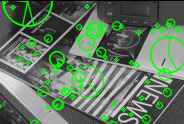
\includegraphics[width=0.9\linewidth]{image.jpg}
	\caption{caption.}
	\label{img:example}
\end{figure}
\chapter{Predicting LIDAR Intensity from RGB and Depth Images}
\section{Setup}
used the bp net it is for depth completion and depth prediction
pix2pix model with modified data loader to get 4 dim. input rgb plus depth
\section{Implementation}
\section{Results}
test run rgb only. depht from depthanything the depth from depthanything v2 and metriv form depthanything v2 6 runs with different solution
\chapter{Conclusion}
\section{Appendix}

\section{References}
bp net work
pix2pix
depth anything v1 2
paper for them 
some for lidar intensity
 

<\chapter{Related Work}

\section{Related 1}

\section{Related 2}
 

% ---------- Anhang ----------

\begin{appendix}
	

\end{appendix}

% ---------- Verzeichnisse ----------

\listoffigures
%\listoftables
%\lstlistoflistings

% ----------------------------

% Erzeugt das Literaturverzeichnis
\printbibliography

% Erzeugt eine Seite mit der Erklaerung
\declaration{nutzung}

\end{document}
